
% Notation for midpoint method stuff
% ============================================================

% notation for "at midpoint"
%% \newcommand{\valueatmidpoint}[1]{\hat{#1}}

% t at midpoint
\newcommand{\thfx}[1]{t_{#1+\half}}
\newcommand{\thf}{\thfx{n}}

% exact y of t at midpoint
\newcommand{\yvhfx}[1]{\yv(\thfx{#1})}
\newcommand{\yvhf}{\yvhfx{n}}

% df/dy matrix
\newcommand{\dfdy}{F}
\newcommand{\dfdyhfx}[1]{\dfdy_{#1+\half}}
\newcommand{\dfdyhf}{\dfdyhfx{n}}

% error due to midpoint approx
\newcommand{\ymiderr}{a_n}

% don't know?
%% \newcommand{\yvhfestx}[1]{\bar{\yv}_{#1}}
%% \newcommand{\yvhfest}{\yvhfestx{n}}


\section{An adaptive implicit-midpoint-method time-integrator}


%*** other names?

%% To make the following derivations more readable we write:
%% \begin{align}
%%   \thf &= \frac{t_n + t_{n+1}}{2}, \notag\\
%%   \yvhf &= \yv(\thf), %\notag\\
%%   %% \yvhfest &= \frac{\yv_{n+1} + \yv_n}{2},
%% \end{align}
%% and we denote derivatives of $\yv$ by $\yv'$ etc.


\subsection{Fixed step implicit midpoint method}

Let $\yv(t)$ be a vector function of time, let $\yv_n$ denote a vector of estimates to $\yv(t)$ at $t = t_n$.
Let $\dtn = t_{n+1} - t_n$ be the (time-)step.
Then given a system of equations of the form
\begin{equation}
  \yv'(t) = \fv(t, \yv(t)),
  \label{eq:43}
\end{equation}
the implicit midpoint method is
\begin{align}
  \yv_{n+1} &= \yv_n + \dtn \fv(\frac{t_{n+1} + t_n}{2}, \frac{\yv_n + \yv_{n+1}}{2}), \notag\\
  &= \yv_n + \dtn \fv(\thf, \frac{\yv_n + \yv_{n+1}}{2}),
  \label{eq:basic-midpoint}
\end{align}
where we have written
\begin{equation}
  \frac{t_{n+1} + t_n}{2} = \thf,
\end{equation}
for readability.

Note that unlike multistep methods (\eg BDF2, AB2) this is valid for both constant and variable step sizes because there is no dependence on previous steps.


\subsection{Derivation of local truncation error}
\label{sec:deriv-local-trunc}

The local truncation error (LTE) of a time integration scheme is the error due a single integration step.
It can be calculated by substituting $\yv_n = \yv(t_n)$ into the approximation for the next time-step then subtracting the result from the exact solution at the next time-step, $\yv(t_{n+1})$.

Using this definition the local truncation error of the midpoint method is
\begin{align}
  \lte^\IMP &= \yv(t_{n+1}) - \yv_{n+1}^\IMP, \notag\\
  &= \yv(t_{n+1}) - \yv(t_n) - \dtn \fv\left( \thf, \frac{\yv(t_n) + \yv_{n+1}^\IMP}{2} \right).
  \label{eq:trunc-start}
\end{align}

We choose to Taylor expand everything about the midpoint, $\thf$, because it reduces the complexity of the result (and allows easier calculations).\footnote{If instead chose to expand about $t_n$ there would be an additional term in $\yv_n''$ in equation~\eqref{eq:trunc-mid}.}
We assume throughout that $\yv(t)$ is ``sufficiently smooth'' to have a Taylor series expansion. Then its Taylor series expansion at $t_{n+1}$ about $\thf$ is given by
\begin{equation}
  \yv(t_{n+1}) = \yv(\thf + \frac{\dtn}{2}) = \yvhf + \frac{\dtn}{2} \yvhf' + \frac{\dtn^2}{8} \yvhf'' + \frac{\dtn^3}{48} \yvhf''' \porder{\dtn^4}.
  \label{eq:taylornp1}
\end{equation}
%% It is well known that the local truncation error of the midpoint method is $\order{\dtn^3}$ (\ie it is second order)\cite{??ds}, so we can safely ignore $\order{\dtn^4}$ terms.
Similarly the expansion at $t_n$ is
\begin{equation}
  \yv(t_n) = \yv(\thf - \frac{\dtn}{2}) = \yvhf - \frac{\dtn}{2} \yvhf' + \frac{\dtn^2}{8} \yvhf'' - \frac{\dtn^3}{48} \yvhf''' \porder{\dtn^4}.
  \label{eq:taylorn}
\end{equation}

Substituting equations~\eqref{eq:taylornp1} and \eqref{eq:taylorn} into equation~\eqref{eq:trunc-start} gives
\begin{equation}
  \lte^\IMP = \yv(t_{n+1}) - \yv_{n+1}^\IMP
  = \frac{\dtn^3}{24} \yvhf'''  + \dtn  \left[ \yvhf'
  - \fv\left( \thf, \frac{\yv(t_n) + \yv_{n+1}}{2} \right) \right]  \porder{\dtn^4}.
  \label{eq:trunc-mid}
\end{equation}

There are two parts to this error: the first term (with $\yv'''_n$) is fairly standard in second order time integrators.
However the second term is more complex, applying a Taylor expansion approach here would result in a Jacobian-like matrix of derivatives of $\fv$ with respect to $\yv$.
Hence we avoid expanding it further.
See Section~\ref{sec:full-imr-lte-calculation} for details of the rest of the Taylor expansion which proves that the midpoint method is indeed a second order method.



\subsection{Construction of an adaptive scheme}

In order to construct an adaptive time integration scheme we must find an easy to compute approximate to the local truncation error \eqref{eq:trunc-mid}.

First, notice that we can rearrange equation~\eqref{eq:basic-midpoint} to get
\begin{equation}
  \fv\left( \thf, \frac{\yv(t_n) + \yv_{n+1}}{2} \right) = \frac{\yv_{n+1} - \yv_n}{\dtn},
\end{equation}
which we can substitute into equation~\eqref{eq:trunc-mid}, leaving
\begin{equation}
  \lte^\IMP = \frac{\dtn^3}{24} \yvhf'''  + \dtn \yvhf' + \yv_n - \yv_{n+1}
  \porder{\dtn^4}.
\end{equation}
To keep algebra simpler we write
\begin{equation}
   \ymiderr = \dtn  \left[ \yvhf'
  - \fv\left( \thf, \frac{\yv(t_n) + \yv_{n+1}}{2} \right) \right] =  \dtn \yvhf' + \yv_n - \yv_{n+1}
\end{equation}

Next we use a second order Adams-Bashforth method as a ``predictor'' to eliminate the difficult-to-estimate $\yvhf'''$ term.
The approach is somewhat similar to that used in some adaptive trapezoid rule algorithms.\cite[p.707]{Gresho-Sani}

\subsubsection{Elimination of $\yvhf'''$ term by Adams-Bashforth Predictor}
The second-order variable time-step Adams-Bashforth method is\cite[p.267]{Gresho-Sani}
\begin{equation}
  \yv_{n+1}^{\AB} = \yv_n + \frac{\dtn^\AB}{2} \left[
    \left (2 + \frac{\dtn^\AB}{\dtx{n-1}^\AB} \right) \yv'_n
    - \frac{\dtn^\AB}{\dtx{n-1}^\AB} \yv'_{n-1}
    \right],
  \label{eq:AB2}
\end{equation}
and its local truncation error is\cite[p.267]{Gresho-Sani}
\begin{equation}
  \lte^{\AB} = \yv(t_{n+1}) - \yv_{n+1}^{\AB}
  = \left( 2 + \frac{3 \dtx{n-1}^\AB}{\dtn^\AB} \right) \frac{(\dtn^\AB)^3}{12} \yv'''(t_n^\AB)
  \porder{\dtn^4}.
  \label{eq:AB2LTE}
\end{equation}

Note that equation~\eqref{eq:trunc-final} involves $\yvhf''' = \yv'''([t_n +t_{n+1}]/2)$ whereas equation~\eqref{eq:AB2LTE} involves $\yv'''(t_n^\AB)$.
Hence to eliminate the derivative we need to ``offset'' the Adams-Bashforth time-steps with respect to the midpoint method such that the $n$th time-step of the AB2 scheme is at the ``midpoint''.
We also require that the $(n+1)$th time-steps be the same in both schemes so that the $\yv(t_{n+1})$ terms on the LHS of the truncation error equations will cancel.
\begin{align}
  t_{n+1}^\AB &= t_{n+1}, \notag\\
  t_n^\AB &= \thf = (t_{n} + t_{n+1})/2  \qquad   (\dtn^\AB = \frac{\dtn}{2}).
  \label{eq:ab2-ts}
\end{align}
The $(n-1)$th step can be chosen freely, we pick
\begin{equation}
  t_{n-1}^\AB = t_n  \qquad   (\dtx{n-1}^\AB = \frac{\dtn}{2} = \dtn^\AB),
\end{equation}
for simplicity.\footnote{Depending on the method used to calculate input values for this step (see Section~\ref{sec:calc-requ-input}) $t_{n-1}^\AB = \thf$ might be preferable. The algebra is more complex but the numerical behaviour appears to be identical.}

With these times the AB2 method \eqref{eq:AB2} becomes
\begin{equation}
   \yv_{n+1}^{\AB} = \yvhf + \frac{\dtn}{4} \left[
     3 \yvhf' - \yv_n' \right],
   \label{eq:AB2-mid}
\end{equation}
and the local truncation error \eqref{eq:AB2LTE} becomes
\begin{equation}
  \lte^\AB = \yv(t_{n+1}) -  \yv_{n+1}^{\AB}
  = \frac{5 \dtn^3}{96} \yvhf''' \porder{\dtn^4}.
\label{eq:AB2-mid-LTE}
\end{equation}

We can eliminate the unknown $\yv(t_{n+1})$ term by subtracting the Adams-Bashforth LTE \eqref{eq:AB2-mid-LTE} from the midpoint method LTE \eqref{eq:trunc-final}
\begin{align}
 - \yv_{n+1}^{\IMP} + \yv_{n+1}^{\AB} &=
   \frac{\dtn^3}{24} \yvhf''' + \ymiderr
  - \frac{5\dtn^3}{96} \yvhf'''
  \porder{\dtn^4}, \notag \\
  - \yv_{n+1}^{\IMP} + \yv_{n+1}^{\AB} &= -\frac{1}{4} \left( \frac{\dtn^3}{24} \yvhf''' \right)
  + \ymiderr
  \porder{\dtn^4},
\end{align}
Rearranging gives us an expression for $\yvhf'''$
\begin{equation}
  \frac{\dtn^3}{24} \yvhf''' = 4 \left[ \yv_{n+1}^\IMP - \yv_{n+1}^{\AB} + a_n \right]  \porder{\dtn^4},
\end{equation}
which can be substituted into equation~\eqref{eq:trunc-final} to give the truncation error
\begin{equation}
  \lte^\IMP = 4 \left[ \yv_{n+1}^\IMP - \yv_{n+1}^{\AB} \right] + 5 a_n
  \porder{\dtn^4}.
  \label{eq:50}
\end{equation}


\subsubsection{Calculation of Required Input Values}
\label{sec:calc-requ-input}

It remains to provide efficient ways of calculating $\yvhf$, $\yv_n'$, $\yvhf'$.
Note that we can't just use the approximation $\yvhf \simeq \frac{\yv(t_n) + \yv_{n+1}}{2}$ because there is an error of order $\dtn^2$ involving $\yvhf''$ (see Section~\ref{sec:full-imr-lte-calculation} for details), which is even harder to calculate than $\yvhf$ itself.
Instead we interpolate the values at the points needed from the known values at integer time steps.

The points $y_n, y_{n-1}, y_{n-2}, \ldots$ can be assumed to be exact in LTE estimation, so these will be the points used for interpolation.
Other known values have an error (typically related to the truncation error) so these will not be used.

If $\fv(t, \yv(t))$ is cheap to calculate, \ie it is given explicitly as in equation~\eqref{eq:43} then additional derivative values could be used as interpolation inputs.
As an additional benefit the location (in time) of these derivatives can be chosen to improve the numerical stability of the interpolation.
However, to remain more general (and in particular to allow the application of this scheme to the Gilbert form of the LLG equation) we avoid additional function evaluations and use only the previous time values.

Barycentric Lagrange seems to be the ``best'' interpolation method.\cite{Berrut2004}
But Hermite with divided differences gives an easy way to get derivatives in scipy implementation so use that for now.
Errors should be the same.

%So as long as the previous $\texttt{npoints}$ time-steps are of comparable size to this one the interpolation will be $\order{\dtn^\texttt{npoints}}$.
%Otherwise it will be $~\order{\dtn \dtx{n-1} \dtx{n-2}\cdots}$.

There are conflicting requirements on the number of points to use for the interpolation ($\texttt{npoints}$). As number of points is increased:
\begin{itemize}
\item Higher power in error term $\order{\dtn^\texttt{npoints}}$.
\item Increases coupling to past values, which can induce oscillations in $\dtn$ (see numerical experiments section ??ds).
\item We need $\texttt{npoints}$ known values before adaptivity can be used.
\end{itemize}
Numerical experiments show that 2 points works best.


%% Numerical experiments show that interpolating using $y_{n+1}^\IMP$ causes an increase in oscillations and strange behaviour, probably because of the truncation error (which is large compared to the interpolation error).
%% We also have estimates for $\yvhf$, $\fv(\thf, \yvhf)$ for all $n \leq n+1$, with low accuracy, probably no way to use these..
%% Unless we use some kind of least squares fitting, probably too expensive.


\subsubsection{Computing the size of the next time-step}
% new

We use a standard method for computing the next time step from the local truncation error and a target local truncation error $\texttt{tol}$:\cite[pg.268]{Gresho-Sani}
\begin{equation}
\dtx{n+1} = \dtn \left( \frac{\texttt{tol}}{\lte^\IMP}  \right) ^{\frac{1}{3}}
\end{equation}


\subsection{Numerical experiments}

To demonstrate the effectiveness of the adaptation scheme we use a simple ODE with known exact solution
\begin{align}
  f(t,y) &= - \beta e^{-\beta t} \sin(\omega t) + \omega e^{-\beta t} \cos(\omega t) \\
  y(0) &= 0
\end{align}
which gives the exact solution
\begin{equation}
  \label{eq:59}
  y(t) = e^{-\beta t} \sin(\omega t).
\end{equation}
The numerical experiments below all use $\omega = 2 \pi$ and $\beta = 0.3$.
The exact solution for this case is shown in Figure~\ref{fig:mp-ode-exact}.
Plots of the solutions given by the various numerical calculations below are all visually indistinguishable from Figure~\ref{fig:mp-ode-exact} (without zooming in) at the tolerances used, so they are not shown.

\begin{figure}[ht!]
  \centering
  \includegraphics[width=0.8\textwidth]
                  {/home/david/Dropbox/programming/simplellg/experiments/exact}
  \caption{A plot of equation~\eqref{eq:59}, the exact solution of our example ODE.}
  \label{fig:mp-ode-exact}
\end{figure}

Figure~\ref{fig:mp-ninterp} shows the step sizes selected with various numbers of interpolation points used.
For larger numbers of interpolation points spurious oscillations begin to appear which are not related to the solution.
??ds mention errors $\propto$ third derivative


This could be due to increased coupling between previous points.
Alternatively it could be due to Runge oscillations (a phenomenon commonly seen in polynomial interpolation when interpolation points are not careful selected), but this is unlikely because the number of points at which the oscillations appear is so low.
\begin{figure}[ht!]
  \centering
  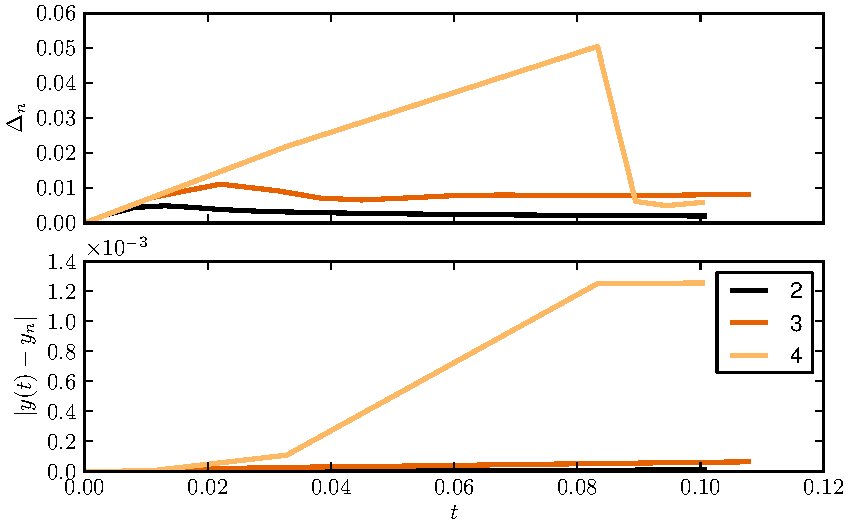
\includegraphics[width=\textwidth]
                  {/home/david/Dropbox/programming/simplellg/experiments/mp_ninterp}
  \caption{Behaviour of adaptive midpoint method using different numbers of interpolation points for a simple ODE. The \texttt{tol} parameter used is $1\E{-4}$.}
  \label{fig:mp-ninterp}
\end{figure}


Figure~\ref{fig:mp-vs-bdf2} shows the performance of the adaptive midpoint scheme derived above compared to a standard adaptive BDF2 scheme.\cite{Gresho-Sani} %pg 715
The step size selection of the adaptive midpoint scheme closely follows that of the BDF2 scheme.
Also of note that the accuracy of the midpoint method is much higher than that of BDF2 for the same step size in this example.
This is due to the fact that for ODEs where $f$ is not a function of $y$ (such as the one used here) the local truncation error of the midpoint method is equivalent to that of the trapezoid rule (see Section~\ref{sec:full-imr-lte-calculation} equation~\eqref{eq:trunc-final}) which has the smallest possible leading coefficient in the local truncation error.\cite{Gresho-Sani} % pg 281

\begin{figure}[ht!]
  \centering
  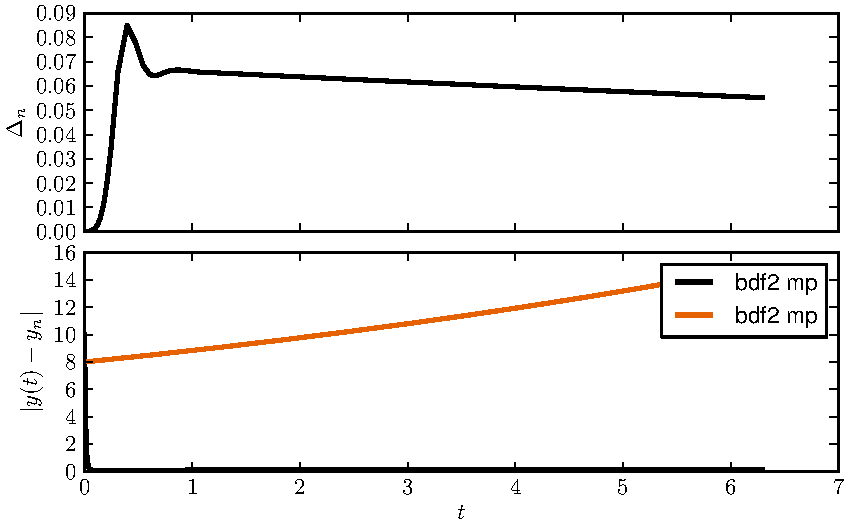
\includegraphics[width=\textwidth]
                  {/home/david/Dropbox/programming/simplellg/experiments/bdf2_vs_mp}
  \caption{Adaptive midpoint (using two interpolation points) vs adaptive BDF2 for a simple ODE. The \texttt{tol} parameter used is $1 \E{-4} $ for both schemes.}
  \label{fig:mp-vs-bdf2}
\end{figure}

Figure~\ref{fig:mp-tols} compares error norm and step sizes for the adaptive midpoint scheme with two interpolation points for varying tolerances.
The midpoint method can be seen to have quadratic convergence by comparing with the $y=x^2$ line shown.
Additionally it can be seen that decreasing the tolerance smoothly decreases the mean error (by smoothly decreasing the mean step size).

\begin{figure}[ht!]
  \centering
  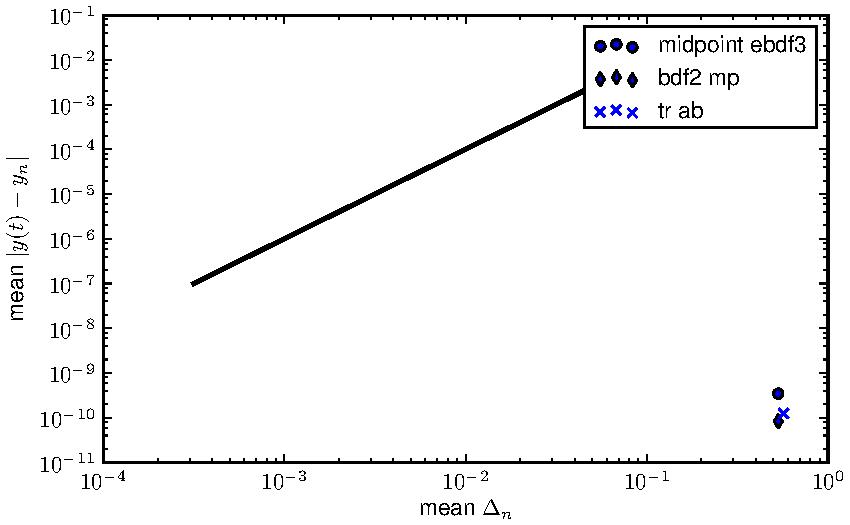
\includegraphics[width=\textwidth]
                  {/home/david/Dropbox/programming/simplellg/experiments/mp_tols}
  \caption{Adaptive midpoint mean dt vs mean error for varying tolerance. The line is $y = x^2$.}
  \label{fig:mp-tols}
\end{figure}


\subsection{Additional Notes}

\subsubsection{Extension to implicit ODEs}
\label{sec:extens-impl-odes}

We sometimes wish to solve a system of equations where $\yv'(t)$ only given implicitly\footnote{This use of ``implicit'' is unrelated to the notion of implicitness in the time integration scheme.} (for example the Gilbert form of the Landau-Lifshitz-Gilbert equation), in this case equation~\eqref{eq:43} becomes
\begin{equation}
  \fv(t, \yv(t), \yv'(t)) = 0.
\end{equation}

We note that equation~\eqref{eq:basic-midpoint} can also be written in the from
\begin{equation}
  \yv'(\thf) = \frac{\yv_{n+1} - \yv_n}{\dtn} =  \fv(\thf, \frac{\yv_n + \yv_{n+1}}{2}).
\end{equation}
So the obvious equivalent for the midpoint method is
\begin{equation}
  \fv(\thf, \frac{\yv_{n+1} + \yv_n}{2}, \frac{\yv_{n+1} - \yv_n}{\dtn}) = 0.
\end{equation}

Also note that we have avoided the requirement for any additional function (\ie $\fv$) evaluations during the estimation of the local truncation error.
Hence everything derived here is equally applicable to implicit ODEs.


\subsubsection{Use of Predictor for Initial Guess}

Often the predictor (i.e. the explicit method used to eliminate the highest derivative of $\yv$) is used to give an initial guess for the non-linear solve.
In fact this appears to be where the term ``Predictor-Corrector'' originates.
This is not possible here because we use $\yv_{n+1}$ in the predictor calculation.
However past experience with Newton's method suggests that using a predictor instead of the value at the previous time $\yv_n$ gives no reduction in the number of Newton steps needed for convergence.\cite{Milan, Matthias}
Hence there is no disadvantage in using $\yv_{n+1}$ in the predictor calculation.

\subsubsection{Suitability of Adams-Bashforth 2 Predictor}

There are a large number of explicit time integration algorithms, here we list the requirements which result in the decision to use AB2 over other possibilities:
\begin{itemize}
\item Must be second order (and no higher), otherwise it cannot be used to eliminate the $\yv'''$ term.

\item Must be calculable without calculating $\yv'$ at points far away from where it is already calculated.
  Otherwise we would need to perform additional separate calculations.
  This would be reasonable if the $\yv'$ is given explicitly, but that is not always the case.
  So we avoid additional $\yv'$ evaluations for increased generality (and in particular for use with the Gilbert form of the LLG equation).

\item Must not reduce to the implicit midpoint rule when shifted to appropriate times and the approximation under any approximations used.
  This is the case for the explicit midpoint rule if we try $\fv(\thf, \yv_n + \dtn \fv(t_n, \yv_n)) \simeq \fv(\thf, \frac{\yv_n + \yv_{n+1}}{2})$.
\end{itemize}

Other second order explicit ODE solvers:
\begin{itemize}
\item Explicit midpoint rule (a.k.a. Verlet, leapfrog method) -- see requirement 3.
\item Heunn's method -- requires a $\yv'$ evaluation at a point determined by a previous evaluation which almost always require a new calculation, see requirement 2. Similarly for any other variants on second order Runge-Kutta methods other than the explicit midpoint rule.
\end{itemize}


Other possibilities:
\begin{itemize}
\item Some sort of explicitised-BDF2? Replace $\yv_{n+1}$ on RHS of expression by $\yv_{n+1}^\IMP$ and calculate explicitly? LTE could be hard to derive... Similar to predictor-corrector methods...
\item Interpolate or FD derivatives further to get values at whatever points are needed. Probably quite a bad loss of accuracy from interpolation.
\end{itemize}


\subsubsection{Full lte calculation of implicit midpoint}
\label{sec:full-imr-lte-calculation}

Continuing from equation~\eqref{eq:trunc-mid} at the end of Section~\ref{sec:deriv-local-trunc}.

In order to be able to cancel terms we now need to Taylor expand $\fv\left( \thf, \frac{\yv(t_n) + \yv_{n+1}}{2} \right)$ in $\yv$ about $\yvhf$.
Hence we need an expansion of the form
\begin{align}
  \fv(\thf, \frac{\yv(t_n) + \yv_{n+1}}{2}) &= \fv(\thf, \yvhf + \dyn),
  \notag \\
  &= \fv(\thf, \yvhf) + \dfdyhf \cdot \dyn  \porder{\dyn^2}
  \label{eq:f-taylor}
\end{align}
where $\dfdyhf = \dfdy(\thf, \yvhf)$ is a \emph{matrix} of partial derivatives of each element of $\fv$ with respect to each element of the vector $\yv$ (\ie almost a Jacobian, except without the time derivative).
Note that the $\fv$ term is multiplied by an additional factor of $\dtn$ in \eqref{eq:trunc-start}, so for this part of the derivation we can drop terms of higher order than $\order{\dtn^2}$ and still retain the same asymptotic accuracy.

We now derive the required correction $\dyn$.
From equation~\eqref{eq:f-taylor} we have
\begin{equation}
  \dyn = \frac{\yv(t_n) + \yv_{n+1}}{2} - \yvhf.
  \label{eq:51}
\end{equation}
However we cannot expand $\yv_{n+1}$ to get $\dyn$ in terms of only values at the midpoint.
So we use the LTE of the midpoint method to rewrite equation~\eqref{eq:51} as
\begin{equation}
  \dyn = \frac{\yv(t_n) + \yv(t_{n+1}) - \lte^\IMP}{2} - \yvhf.
\end{equation}
Substituting in the Taylor expansions for $\yv(t_n)$ and $\yv(t_{n+1})$ about $\thf$ (from equations~\eqref{eq:taylornp1} and \eqref{eq:taylorn}) gives
\begin{align}
  \dyn &= \yvhf + \frac{\dtn^2}{8} \yvhf'' - \yvhf - \frac{1}{2} \lte^\IMP \porder{\dtn^4} \notag\\
  &= \frac{\dtn^2}{8} \yvhf'' - \frac{1}{2} \lte^\IMP \porder{\dtn^4}
  \label{eq:dy-value}
\end{align}



Substituting the above value for $\dyn$ into the Taylor series expansion of $\fv$ from \eqref{eq:f-taylor} gives
\begin{equation}
  \fv(\thf, \frac{\yv(t_n) + \yv_{n+1}}{2}) = \yvhf'
  + \frac{\dtn^2}{8} \dfdyhf \cdot \yvhf'' - \frac{1}{2} \dfdyhf \cdot \lte^\IMP \porder{\dtn^4}
  . \label{eq:fy-taylor}
\end{equation}
and using \eqref{eq:fy-taylor} in \eqref{eq:trunc-mid} gives the local truncation error
\begin{align}
  (I + \frac{\dtn}{2}\dfdyhf) \cdot\lte^\IMP
  &= \dtn \yvhf' + \frac{\dtn^3}{24} \yvhf'''
  - \dtn \yvhf'
  - \frac{\dtn^3}{8} \dfdyhf \cdot \yvhf'' \porder{\dtn^4}
  \notag \\
  &= \frac{\dtn^3}{24} \left[\yvhf''' - 3 \dfdyhf \cdot \yvhf'' \right]
  \porder{\dtn^4}.
  \label{eq:trunc-implicit-form}
\end{align}

Using a geometric series representation we can show that if all eigenvalues of  $-\frac{\dtn}{2}\dfdyhf$ are s.t. $\abs{\lambda} < 1$\cite{??ds} (which will always be true for some ``small enough'' $\dtn$) then
??ds can we divide by the largest eigenvalue somewhere to do this?
\begin{equation}
  (I + \frac{\dtn}{2}\dfdyhf)^{-1} = I - \frac{\dtn \dfdyhf}{2}  \porder{\dtn^2},
\end{equation}
and so\footnote{Assuming that $\dfdyhf$ is not inversely proportional to $\dtn$.}
\begin{equation}
  \lte^\IMP = \frac{\dtn^3}{24} \left[\yvhf''' - 3 \dfdyhf \cdot \yvhf'' \right]
  \quad +\order{\dtn^4}.
  \label{eq:trunc-final}
\end{equation}



\section{Application of the adaptive midpoint method to micromagnetics}

%*** Banas' work

\subsection{Why use the midpoint method}

The midpoint method is known to be especially effective for micromagnetics problems \cite{DAquino2005}.
The continuous, non-dimensional form of the Landau-Lifshitz-Gilbert equation is
\begin{equation}
  \label{eq:llg-prop-form}
  \dmdt = - \mv \times( \hv - \dampc \dmdt),
\end{equation}

It has certain properties:
\begin{itemize}
\item conserves magnetisation length
\item dissipates energy at a rate determined by alpha (as defined by a Rayleigh dissipation functional)
\item conserves energy at zero damping.
\end{itemize}

Clearly it is advantageous for a time discretisation method to preserve these properties.
Midpoint method conserves them (demonstrated below), most other time discretisation schemes don't.

In addition to these properties the midpoint method is:
\begin{itemize}
\item second order accurate -- typically considered good enough for pdes (higher orders would require expensive high order spatial discretisation to be effective, generally better to just do h-refinement instead) \cite{Matthias}
\item ??ds-stable - think it's A-stable? \cite{??ds} -- so appropriate for stiff problems, llg is stiff in some/most cases\cite{??ds}.
\end{itemize}

Since the midpoint method is a single step method there is no dependence on $\dtx{n-1}$ (unlike, for example, BDF2) and so no change in these properties is expected when going from fixed to varying time step sizes.

\subsection{Properties of continuous Landau-Lifshitz-Gilbert equation}
\label{sec:prop-cont-llg}

We will use the identity
\begin{equation}
  \label{eq:dot-cross-id}
  \ip{\av}{\av \times \bv} = 0,
\end{equation}
which is true for all inner products because $\av \times \bv$ is perpendicular to $\av$ by the definition of the cross product.

Conservation of magnetisation length can be shown by taking the dot product (scalar product, pointwise inner product) with $\mv$ on both sides of~\eqref{eq:llg-prop-form} and using~\eqref{eq:dot-cross-id} to get
\begin{equation}
  \label{eq:56}
  \mv \cdot \dmdt = 0.
\end{equation}
Hence the change in $\mv$ is always perpendicular to $\mv$ so length is conserved.

The energy change properties can be examined similarly by taking the inner product
\begin{equation}
  \ip{u}{v} = \int_\magd u v \d\magd
\end{equation}
with $\hv - \dampc \dmdt$ on both sides of~\eqref{eq:llg-prop-form} and using~\eqref{eq:dot-cross-id} to get
\begin{equation}
  \label{eq:58}
  \ip{\hv}{\dmdt} - \dampc \ip{\dmdt}{\dmdt} = 0.
\end{equation}
Using the fact that $\hv = -\vd{\e}{\mv}$ and the chain rule for variational derivatives we get \cite{??ds}
\begin{align*}
  \pd{\e[\mv(\xv, t), t]}{t} &= \ip{\vd{e}{\mv}}{\dmdt} - \ip{\pd{\happ}{t}}{\mv} \\
             &= -\ip{\hv}{\dmdt} - \ip{\pd{\happ}{t}}{\mv},
\end{align*}
and so
\begin{equation}
  \ip{\hv}{\dmdt} = -\vd{\e}{t} - \ip{\pd{\happ}{t}}{\mv}.
\end{equation}

Substituting this into equation~\eqref{eq:58} gives us
\begin{equation}
  \label{eq:energy-decay}
  \vd{\e}{t} = -\dampc \ip{\dmdt}{\dmdt} - \ip{\pd{\happ}{t}}{\mv}.
\end{equation}

Equation~\eqref{eq:energy-decay} shows that under constant applied field the energy of the system is always decreasing by an amount proportional to $\dampc$.
In fact this relationship is the Rayleigh dissipation functional used as the basis for the derivation of the Gilbert form of the LLG.\cite{Gilbert2004}
For non-constant applied fields the change in the Zeeman energy is added which may increase or decrease the energy depending on how the field is changed. % field moves towards m -> decrease, away -> increase. For non-spatially constant this is averaged over space in some sense by the inner product.


\subsection{Properties of midpoint method LLG discretisation}
\label{sec:prop-midp-meth}

??ds discuss which inner products/norms are used where

As noted in Section~\ref{sec:extens-impl-odes} the midpoint method is defined by the following substitutions
\begin{align}
  \label{eq:55}
  \pd{\mv}{t} &= \frac{\mv_{n+1} - \mv_n}{\dtn}, \\
  \mv &= \frac{\mv_{n+1} + \mv_n}{2}, \\
  t &=  \frac{t_{n+1} + t_n}{2}.
\end{align}

The special conservation properties of the midpoint method discretisation of the Landau-Lifshitz-Gilbert equation come from the fact that for any symmetrical linear operator $\ell$
\begin{align}
  \label{eq:54}
  \ip{\ell \left[ \mv_{n+\half} \right]}{ \pd{\mv}{t} \lvert_{n+\half}}
  &= \frac{1}{2\dtn} \left[
    (\mv_{n+1} , \ell \mv_{n+1})
    + (\mv_{n+1} , \ell \mv_{n})
    - (\mv_{n} , \ell \mv_{n+1})
    - (\mv_{n} , \ell \mv_{n})
    \right] \notag\\
  &= \frac{1}{2\dtn} \left[
    (\mv_{n+1} , \ell \mv_{n+1})
    - (\mv_{n} , \ell \mv_{n})
    \right].
\end{align}

In particular for the identity operator, $\mv \in \real$ and $(\av, \bv) = \av \cdot \bv$ we have
\begin{equation}
  \label{eq:52}
  \mv \cdot \pd{\mv}{t}  = \frac{1}{2\dtn} (\norm{\mv_{n+1}}^2 - \norm{\mv_{n}}^2 ).
\end{equation}
Substituting this into equation~\eqref{eq:56} gives
\begin{equation}
  \abs{\mv_{n+1} }^2 - \abs{\mv_{n}}^2 = 0 \quad \forall \xv \in \magd
\end{equation}
\ie conservation of magnetisation length.

??ds operators below need checking, dAquino is only concerned with FD...

The time-discretised effective field can be represented as a symmetrical linear operator on magnetisation:\cite{DAquino2005}
\begin{equation}
  \label{eq:hop}
  \hv_n(\xv) = \hop [\mv_n(\xv)] + \happ(\xv, t_n).
\end{equation}
The energy can be written using this operator as
\begin{equation}
  \label{eq:energy-hop}
  \e_n = \frac{1}{2} \ip{\mv_n}{\hop[\mv_n] + \happ(\xv,t_n)}.
\end{equation}

Substituting the midpoint approximation and equation~\eqref{eq:hop} into \eqref{eq:58} leaves
\begin{align}
  \label{eq:60}
  &\ip{ \pd{\mv}{t} \lvert_{n+\half}}{\hop \left[\mv_{n+\half} \right]} + \ip{\frac{\mv_{n+1} - \mv_n}{\dtn}}{\happ(\xv,t_{n+\half})} \\
  &= \dampc \ip{\frac{\mv_{n+1} - \mv_n}{\dtn}}{\frac{\mv_{n+1} - \mv_n}{\dtn}}.
\end{align}
We use a midpoint approximation for the applied field to allow us to cancel terms later:
\begin{equation}
  \label{eq:happ-midpoint}
  \happ(\xv,t_{n+\half}) = \frac{\happ(\xv, t_{n+1}) + \happ(\xv, t_n)}{2} + \order{\dtn^2 \spd{\happ}{t}}.
\end{equation}
Combining equations~\eqref{eq:60}, \eqref{eq:happ-midpoint} and the identity~\eqref{eq:54} gives us
\begin{align}
  &\frac{\ip{\mv_{n+1}}{\hop \left[\mv_{n+1} \right] + \happ(\xv, t_{n+1})}
    - \ip{\mv_{n}}{\hop \left[\mv_{n} \right] + \happ(\xv, t_n)}
    }{2\dtn} \notag\\
  &= \dampc \norm{\frac{\mv_{n+1} - \mv_n}{\dtn}}^2
  + \order{\dtn^2 \spd{\happ}{t}}.
\end{align}
After substitution of the energy from~\eqref{eq:energy-hop} this leaves
\begin{equation}
  \frac{\e_{n+1} - \e_n}{\dtn}
  = \dampc \norm{\frac{\mv_{n+1} - \mv_n}{\dtn}}^2
  + \order{\dtn^2 \spd{\happ}{t}}.
\end{equation}
Hence with (piecewise) linear applied fields the energy loss is exactly correct.

It should be noted that the above properties are only true up to the accuracy with which we solve the LLG. Since the LLG is non-linear this is typically the Newton tolerance.


\subsection{Numerical Experiments}

In this section we present numerical experiments showing that the adaptive midpoint method retains the conservation properties of the fixed step midpoint method.

\subsection{Discussion}

\subsubsection{Extension to pdes}

We have done some initial work using adaptive midpoint for the non-spatially constant LLG (\ie a pde) which works well for fully implicit problems.

Unfortunately the energy/damping conservation properties require the entire calculation to be performed implicitly.
This is incompatible with the semi-implicit FEM/BEM method for magnetostatic field calculations,\cite{Koehler1997} which is used in the current implementation of our model.
However d'Aquino \etal demonstrated an efficient, fully implicit finite difference LLG solver using the fixed step midpoint method\cite{DAquino2005}.
Such a solver should be easy to modify to use the adaptive midpoint method.

The conservation of magnetisation length by the midpoint method does not require a fully implicit calculation as demonstrated by Spargo \etal\cite{Spargo2003a}.
Hence the adaptive midpoint method could be used to construct a semi-implicit magnetisation length conserving scheme with purely numerical time adaptivity, with the advantages discussed in Section~\ref{sec:altern-time-adapt}.


\subsubsection{Alternative time adaptivity methods in micromagnetics}
\label{sec:altern-time-adapt}

In cases where the damping is not exact the effective damping can be used as an error estimator, as proposed by Albuquerque \etal\cite{Albuquerque2001}
??ds The disadvantage of this method (aside from the obvious requirement that the damping be inexact) is that, depending on the discretisation used, the error estimator may be unable to distinguish between insufficient space refinement and insufficient time refinement.
In particular this is the case when the solution is not completely divided into separate effective field calculations and pointwise time integration, such as in a typical Galerkin finite element model.

Rigorous time error estimates for the LLG with limited effective field terms with a certain discretisation method were proven and used to perform adaptive refinement of midpoint method time steps by Ban̆as.\cite{Banas-thesis}
By comparison our adaptive method is much more general in that it can be applied to any differential equation and any discretisation scheme which uses the method of lines for time.


\subsubsection{Symplecity}

??ds I basically have no idea about this stuff.

The fixed step midpoint method is ``almost symplectic'' for the LLG equation with zero damping (Hamiltonian structure is preserved up to a small error).\cite{Austin1993}
However it is well known that most adaptive schemes cannot be symplectic\cite{Iserles2009} % pg. 91
so we do not discuss this area further.


\subsection{Future work}

%*** Does adaptivity trail off eventually like trapazoid?

Testing with pdes.



%%% Local Variables:
%%% mode: latex
%%% TeX-master: "./main"
%%% End:
